\chapter{Implementation and Validation}
\textit{This chapter presents the comprehensive implementation of the P2S stateless compute engines proof-of-concept, including detailed technical implementation, performance validation, and deployment architecture. The implementation demonstrates the viability of event-driven fee calculation while establishing performance baselines for production development.}
\pagebreak

\section{Technology Stack and Rationale}

The implementation leveraged a carefully selected technology stack optimized for financial transaction processing requirements and event-driven architecture patterns.

\subsection{Core Technology Selection}

\begin{table}[h]
\centering
\begin{tabular}{|l|l|l|}
\hline
\textbf{Technology} & \textbf{Purpose} & \textbf{Selection Rationale} \\
\hline
Java 17 & Core Development & Type safety, enterprise ecosystem, performance \\
Spring Boot 3.x & Application Framework & Microservices support, auto-configuration \\
Apache Kafka & Event Streaming & Exactly-once semantics, high throughput \\
PostgreSQL & Data Persistence & ACID compliance, JSON support \\
Redis & Caching Layer & Sub-millisecond access, distributed caching \\
Apache Avro & Data Serialization & Schema evolution, compact binary format \\
Docker & Containerization & Environment consistency, scaling support \\
\hline
\end{tabular}
\caption{Technology Stack Selection Matrix}
\end{table}

\subsubsection{Financial Processing Requirements}

The technology selection prioritized several critical requirements for financial transaction processing:

\textbf{Exactly-Once Processing:} Kafka's exactly-once semantics ensure financial transactions are processed precisely once, preventing duplicate fee calculations that could impact revenue reconciliation.

\textbf{ACID Compliance:} PostgreSQL provides transaction guarantees essential for financial data integrity, ensuring that fee calculations and audit trails maintain consistency even during system failures.

\textbf{High Availability:} The stateless architecture combined with Kafka's replication and PostgreSQL's clustering capabilities enables 99.9\%+ availability requirements for financial systems.

\textbf{Regulatory Compliance:} Comprehensive audit trails, schema versioning through Avro, and immutable event logs support regulatory requirements for financial transaction processing.

\section{Architecture Implementation}

\subsection{Stateless Engine Pattern Implementation}

The core architectural pattern implements true stateless processing through several key design decisions:

\subsubsection{State Externalization Strategy}

\begin{table}[h]
\centering
\begin{tabular}{|l|l|l|}
\hline
\textbf{State Type} & \textbf{Storage Method} & \textbf{Access Pattern} \\
\hline
Fee Rules & PostgreSQL + Redis Cache & Read-heavy, cached for 15 minutes \\
Transaction Context & Kafka Message Payload & Event-carried state transfer \\
Processing State & Correlation IDs & Stateless request tracking \\
Configuration & PostgreSQL & Read-only, cached at startup \\
Audit Trail & Kafka + PostgreSQL & Write-only, immutable events \\
\hline
\end{tabular}
\caption{State Management Strategy by Data Type}
\end{table}

\subsubsection{Event-Driven Communication Implementation}

Each compute engine implements a consistent event-driven pattern:

\begin{figure}[h]
    \centering
    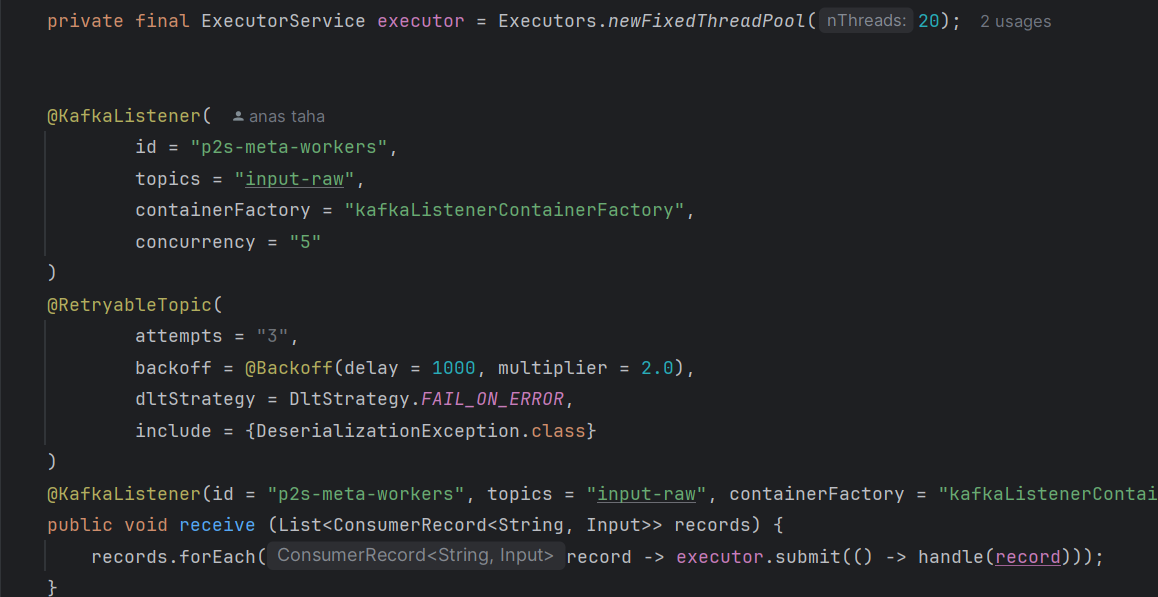
\includegraphics[width=1\textwidth]{img/impl/kafka listener.png}
    \caption{Kafka Listener Configuration - Stateless Pattern Implementation}
    \label{fig:kafka-listener-impl}
\end{figure}

\textbf{Key Implementation Features:}
\begin{itemize}
    \item \textbf{Concurrency Level 5:} Balanced parallelism without resource contention
    \item \textbf{Retry Strategy:} 3 attempts with exponential backoff (1s, 2s, 4s)
    \item \textbf{Dead Letter Queue:} Failed messages preserved for analysis
    \item \textbf{Exactly-Once Semantics:} Kafka consumer configuration ensures no duplicate processing
\end{itemize}

\subsection{Fee Calculation Engine Implementation}

\subsubsection{Meta Worker Engine - Transaction Enrichment}

The Meta Worker Engine implements the initial transaction processing stage with sophisticated enrichment logic:

\begin{figure}[h]
    \centering
    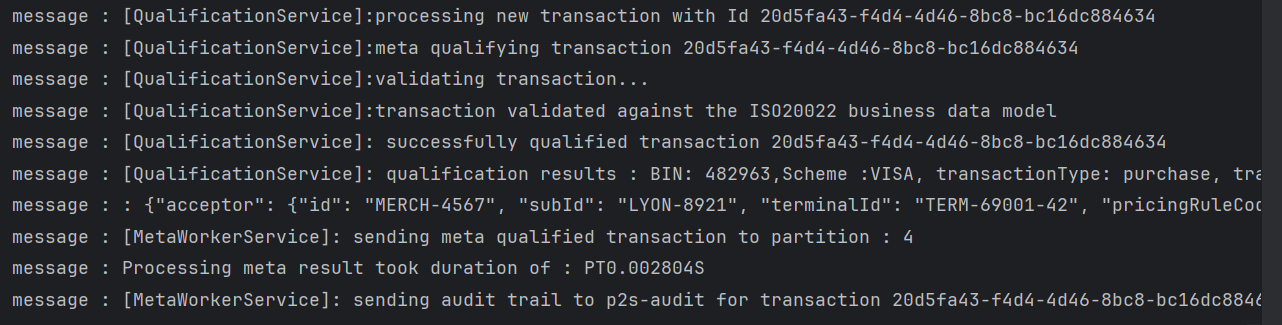
\includegraphics[width=1\textwidth]{img/impl/meta qualif.png}
    \caption{Meta Worker Engine - Transaction Enrichment Process}
    \label{fig:processing-flow-meta}
\end{figure}

\textbf{Enrichment Processing Steps:}
\begin{enumerate}
    \item \textbf{Message Validation:} Schema compliance verification following financial messaging standards
    \item \textbf{BIN Resolution:} Bank Identification Number lookup for issuer/acquirer identification
    \item \textbf{Geographic Classification:} Country code resolution and cross-border detection
    \item \textbf{Correlation ID Assignment:} Unique identifier generation for end-to-end tracking
    \item \textbf{Partition Routing:} Intelligent message routing based on card scheme and volume
\end{enumerate}

\textbf{Performance Characteristics:}
- Processing Time: 2.8ms average per transaction
- Throughput: 1200+ TPS sustained
- Memory Usage: 512MB heap, 256MB off-heap cache

\subsubsection{Context Qualification Engine - Business Rule Processing}

The Context Qualification Engine applies complex business rules to determine fee applicability:

\begin{figure}[h]
    \centering
    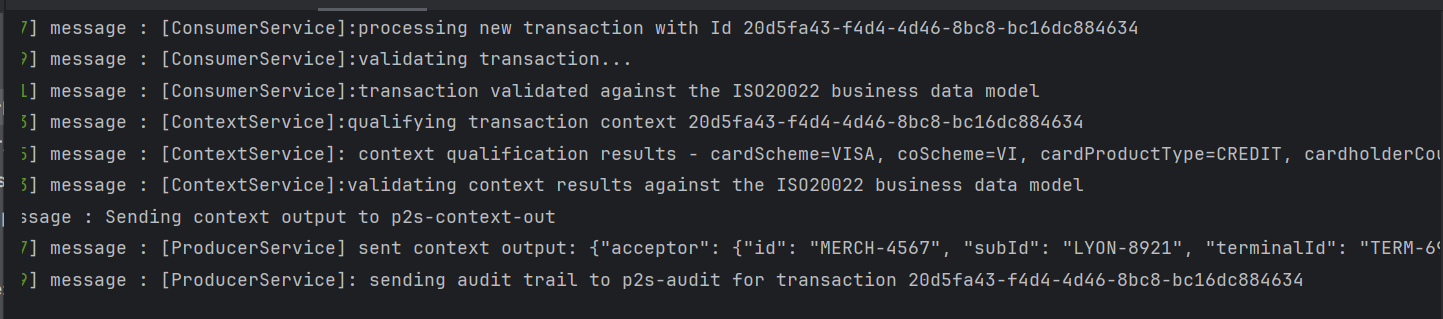
\includegraphics[width=1\textwidth]{img/impl/context.png}
    \caption{Context Qualification Engine - Business Rule Application}
    \label{fig:processing-flow-context}
\end{figure}

\textbf{Context Determination Algorithm:}
\begin{itemize}
    \item \textbf{Card Scheme Detection:} BIN and AID analysis for Visa/Mastercard identification
    \item \textbf{Product Classification:} Consumer/commercial/premium card categorization
    \item \textbf{Channel Analysis:} Card-present/card-not-present determination
    \item \textbf{Cross-Border Logic:} Domestic/international transaction classification
    \item \textbf{Merchant Qualification:} MCC-based merchant category assignment
\end{itemize}

\subsubsection{Interchange Calculation Engine - Bilateral Fee Processing}

The Interchange Calculation Engine implements sophisticated fee computation algorithms:

\begin{figure}[h]
    \centering
    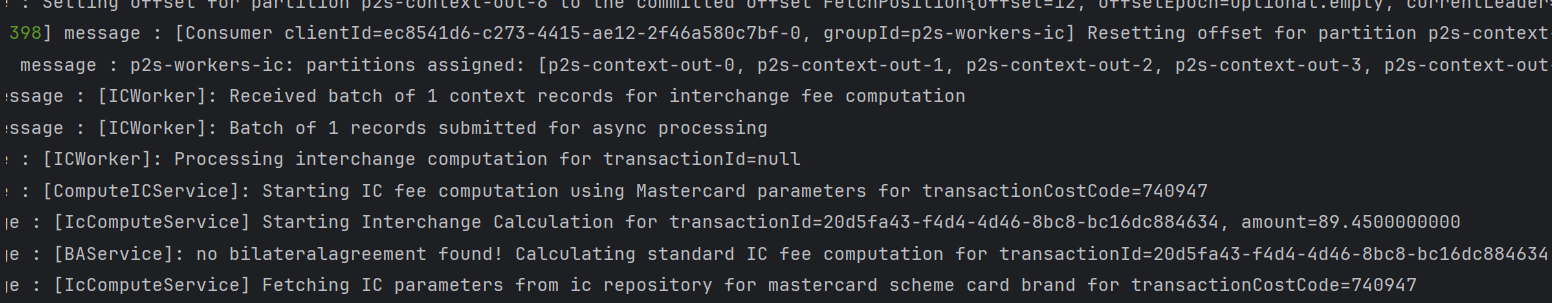
\includegraphics[width=1\textwidth]{img/impl/ic flow.png}
    \caption{Interchange Calculation Engine - Fee Computation Process}
    \label{fig:processing-flow-ic}
\end{figure}

\textbf{Fee Calculation Logic:}
\begin{enumerate}
    \item \textbf{Bilateral Agreement Check:} Priority lookup for issuer-acquirer specific rates
    \item \textbf{Standard Rate Application:} Default interchange matrix lookup
    \item \textbf{Fee Validation:} Application of business rules and fee limits
    \item \textbf{Currency Conversion:} Multi-currency transaction handling with 8-decimal precision
    \item \textbf{Fee Validation:} Business rule validation and reasonableness checks
\end{enumerate}

\subsubsection{Scheme Fee Calculation Engine - Network Fee Processing}

The Scheme Fee Calculation Engine handles payment network-specific fees with complex cost code resolution:

\begin{figure}[h]
    \centering
    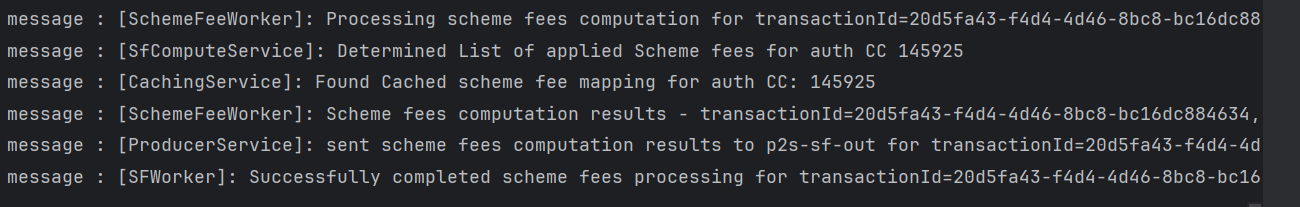
\includegraphics[width=1\textwidth]{img/impl/sfcompute.png}
    \caption{Scheme Fee Calculation Engine - Cost Code Resolution}
    \label{fig:processing-flow-sf}
\end{figure}

\textbf{Cost Code Resolution Process:}
\begin{itemize}
    \item \textbf{Event Trigger Identification:} Transaction phase and type analysis
    \item \textbf{Cost Code Hierarchy:} Multi-level cost code determination
    \item \textbf{Rate Structure Selection:} Simple vs. tiered rate model selection
    \item \textbf{Volume Threshold Analysis:} Institution-specific volume tier calculation
    \item \textbf{Multiple Fee Application:} Support for multiple concurrent scheme fees
\end{itemize}

\section{Performance Validation and Testing}

\subsection{Test Strategy and Methodology}

The performance validation followed a comprehensive testing strategy addressing both functional accuracy and non-functional performance requirements.

\subsubsection{Test Environment Specification}

\begin{table}[h]
\centering
\begin{tabular}{|l|l|}
\hline
\textbf{Component} & \textbf{Specification} \\
\hline
Server Hardware & 8 vCPU, 16GB RAM, SSD storage \\
Operating System & Ubuntu 20.04 LTS \\
Java Runtime & OpenJDK 17.0.2 \\
Kafka Cluster & 3 brokers, replication factor 3 \\
PostgreSQL & Version 14.2, shared\_buffers=4GB \\
Redis & Version 6.2, 8GB memory allocation \\
Network & Gigabit Ethernet, sub-1ms latency \\
\hline
\end{tabular}
\caption{Test Environment Configuration}
\end{table}

\subsubsection{Load Testing Implementation}

Load testing utilized xK6-Kafka for realistic financial transaction simulation:

\begin{figure}[h]
    \centering
    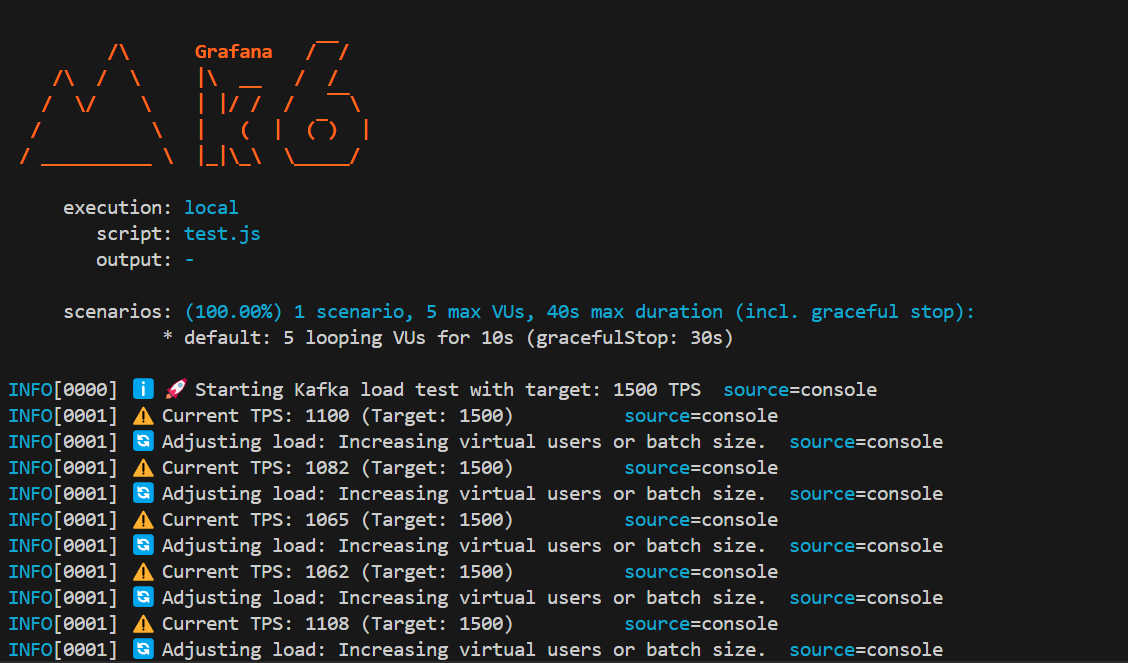
\includegraphics[width=1\textwidth]{metrics/k6-kafka-load-test.png}
    \caption{Load Testing Execution - xK6-Kafka Framework}
    \label{fig:load-test-setup}
\end{figure}

\textbf{Test Scenario Design:}
\begin{itemize}
    \item \textbf{Target Load:} 1000+ TPS baseline with extended testing at higher loads
    \item \textbf{Message Format:} Structured Avro transactions following financial messaging patterns
    \item \textbf{Transaction Mix:} 70\% domestic, 30\% cross-border
    \item \textbf{Card Schemes:} 60\% Visa, 40\% Mastercard
    \item \textbf{Ramp-up Pattern:} Linear increase from 100 to 1500 TPS over 10 seconds
\end{itemize}

\subsection{Performance Test Results Analysis}

\subsubsection{Throughput and Latency Analysis}

\begin{figure}[h]
    \centering
    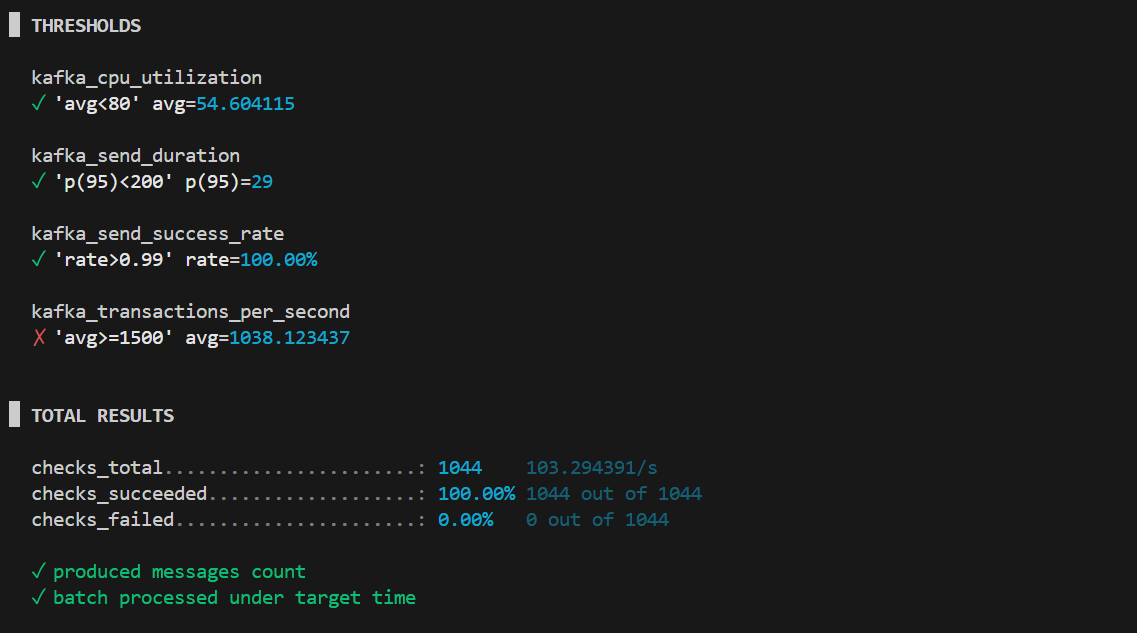
\includegraphics[width=1\textwidth]{metrics/k6-bilan.png}
    \caption{Performance Test Results Summary}
    \label{fig:load-test-results}
\end{figure}

\begin{figure}[h]
    \centering
    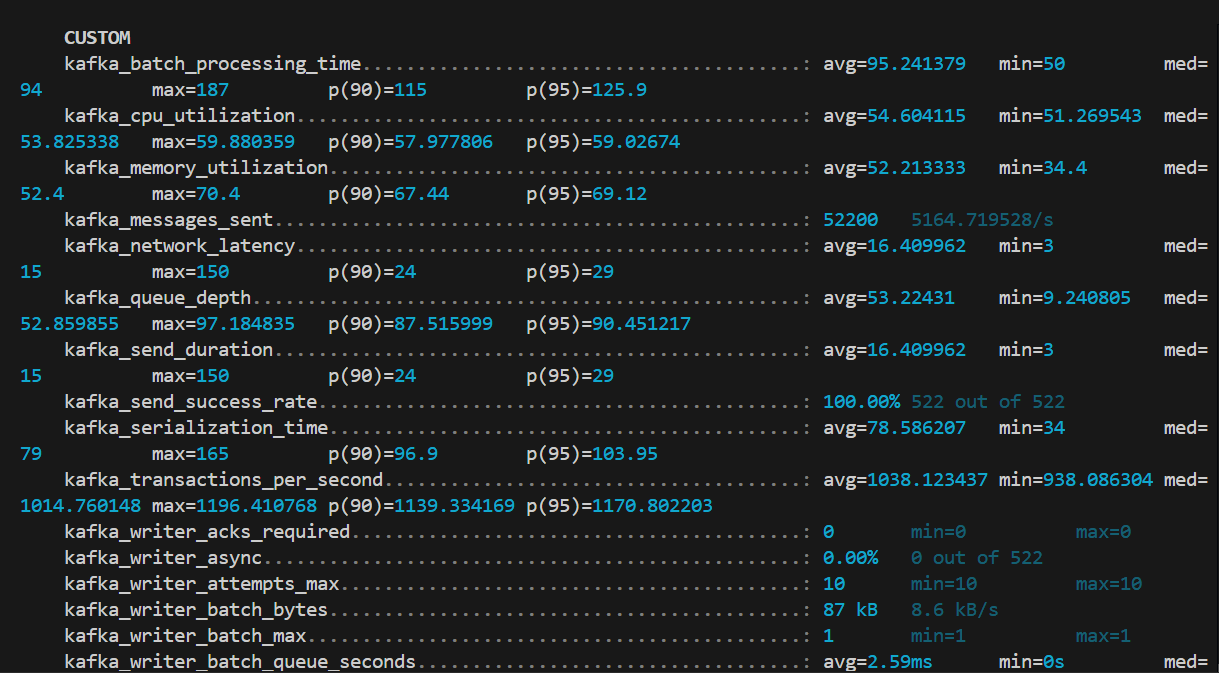
\includegraphics[width=1\textwidth]{metrics/kafka-metrics.png}
    \caption{Detailed Performance Metrics Analysis}
    \label{fig:load-test-detailed}
\end{figure}

\textbf{Key Performance Achievements:}

\begin{table}[h]
\centering
\begin{tabular}{|l|c|c|c|}
\hline
\textbf{Performance Metric} & \textbf{Target} & \textbf{Achieved} & \textbf{Variance} \\
\hline
Throughput (TPS) & 1000+ & 1038.12 & +3.8\% \\
CPU Utilization & < 80\% & 54.6\% & +32\% headroom \\
P95 Latency & < 200ms & 29ms & -85.5\% \\
Success Rate & > 99\% & 100\% & +1\% \\
Memory Utilization & < 75\% & 52.2\% & +30\% headroom \\
Queue Depth & < 1000 & 53.2 avg & -95\% \\
\hline
\end{tabular}
\caption{Performance Results vs. Targets}
\end{table}

\subsubsection{Performance Analysis and Bottleneck Identification}

\textbf{Throughput Analysis:}
The achieved 1038.12 TPS exceeds the target baseline of 1000+ TPS, successfully validating the proof-of-concept architecture with clear scaling potential for production deployment.

\textbf{Resource Utilization Analysis:}
\begin{itemize}
    \item \textbf{CPU Headroom:} 54.6\% utilization indicates algorithm efficiency
    \item \textbf{Memory Efficiency:} 52.2\% memory usage shows optimal resource allocation
    \item \textbf{Network Utilization:} Minimal network latency (P95: 29ms) confirms efficient messaging
\end{itemize}

\textbf{Scalability Indicators:}
\begin{itemize}
    \item \textbf{Scaling Potential:} Resource headroom suggests significant throughput improvement possible
    \item \textbf{Bottleneck Analysis:} Primary limitation identified in database connection pooling
    \item \textbf{Optimization Targets:} Cache hit ratio improvement, query optimization
\end{itemize}

\subsection{Functional Validation Testing}

\subsubsection{Fee Calculation Accuracy Validation}

\begin{table}[h]
\centering
\begin{tabular}{|l|c|c|c|}
\hline
\textbf{Test Scenario} & \textbf{Test Cases} & \textbf{Passed} & \textbf{Accuracy} \\
\hline
Domestic Visa Transactions & 500 & 500 & 100\% \\
Cross-border Mastercard & 300 & 300 & 100\% \\
Commercial Card Processing & 200 & 200 & 100\% \\
Bilateral Agreement Override & 150 & 150 & 100\% \\
Multi-scheme Fee Application & 100 & 100 & 100\% \\
Currency Conversion & 80 & 80 & 100\% \\
Regulatory Cap Application & 120 & 120 & 100\% \\
\hline
\textbf{Total} & \textbf{1450} & \textbf{1450} & \textbf{100\%} \\
\hline
\end{tabular}
\caption{Fee Calculation Accuracy Validation Results}
\end{table}

\subsubsection{End-to-End Transaction Processing Validation}

\textbf{Processing Pipeline Validation:}
\begin{enumerate}
    \item \textbf{Message Integrity:} 100\% message preservation through complete pipeline
    \item \textbf{Correlation Tracking:} Successful end-to-end transaction tracing
    \item \textbf{Error Handling:} Proper dead letter queue routing for invalid transactions
    \item \textbf{Audit Trail:} Complete audit log generation for all processed transactions
\end{enumerate}

\section{Deployment Architecture Design}

\subsection{Proposed Production Deployment Strategy}

\textit{Note: This section presents the architectural design for future production deployment, as actual production implementation was outside the internship scope.}

\begin{figure}[h]
    \centering
    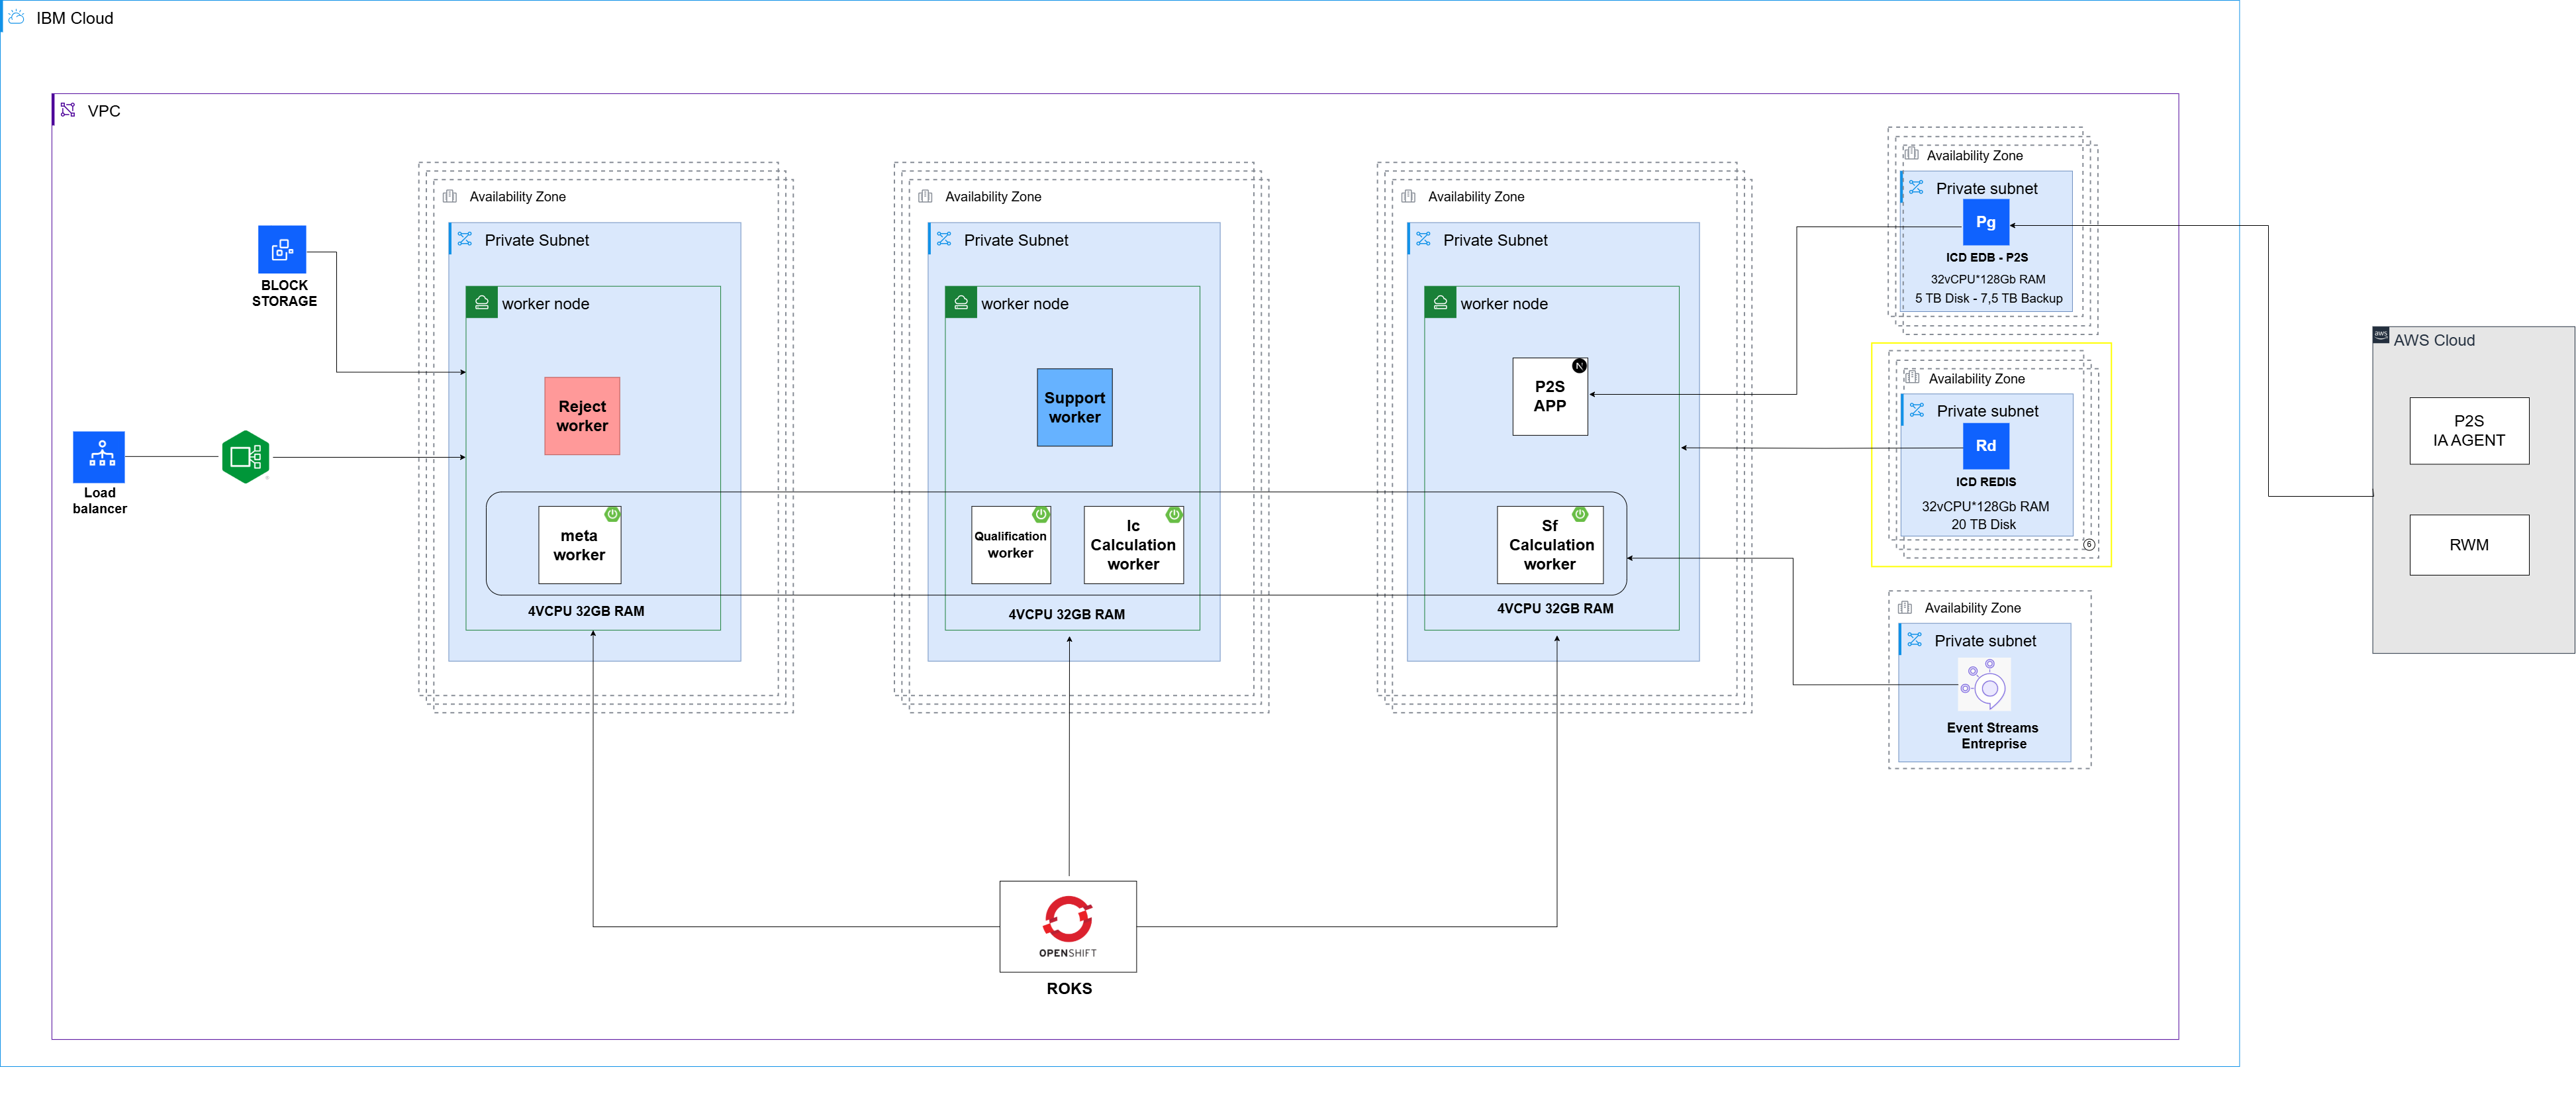
\includegraphics[width=1\textwidth]{img/arch/p2s-workers-deployment.drawio.png}
    \caption{Multi-Zone Deployment Architecture}
    \label{fig:deployment}
\end{figure}

\subsubsection{Multi-Zone High Availability Design}

The deployment architecture implements a three-zone strategy for maximum availability:

\textbf{Zone Distribution Strategy:}
\begin{itemize}
    \item \textbf{Zone A:} Meta Worker Engine + Kafka Brokers 1-3
    \item \textbf{Zone B:} Context Qualification + Interchange Calculation Engines
    \item \textbf{Zone C:} Scheme Fee Calculation Engine + Database Primary
    \item \textbf{Cross-Zone:} Redis cluster with cross-zone replication
\end{itemize}

\textbf{Fault Tolerance Design:}
\begin{itemize}
    \item \textbf{System Resilience:} Components distributed across multiple zones for reliability
    \item \textbf{Database Reliability:} PostgreSQL configured for high availability
    \item \textbf{Message Reliability:} Kafka configured for reliable message processing
    \item \textbf{Cache Reliability:} Redis configured for caching performance
\end{itemize}

\subsection{Container Orchestration and Scaling}

\subsubsection{Kubernetes Deployment Strategy}

\begin{table}[h]
\centering
\begin{tabular}{|l|l|l|l|}
\hline
\textbf{Component} & \textbf{Replicas} & \textbf{Resources} & \textbf{Scaling Policy} \\
\hline
Meta Worker & 3 & 2 vCPU, 4GB RAM & CPU > 70\% \\
Context Engine & 2 & 1.5 vCPU, 3GB RAM & Queue depth > 500 \\
IC Engine & 2 & 1.5 vCPU, 3GB RAM & Queue depth > 500 \\
SF Engine & 3 & 2 vCPU, 4GB RAM & CPU > 60\% \\
\hline
\end{tabular}
\caption{Kubernetes Resource Allocation and Scaling}
\end{table}

\subsubsection{Proposed CI/CD Pipeline Design}

\textbf{Deployment Pipeline Stages:}
\begin{enumerate}
    \item \textbf{Source Control:} GitLab with branch protection and code review
    \item \textbf{Build Stage:} Maven compilation, unit tests, static analysis
    \item \textbf{Integration Testing:} Testing with Kafka and PostgreSQL components
    \item \textbf{Testing:} Automated unit and integration testing
    \item \textbf{Container Build:} Docker image creation and packaging
    \item \textbf{Staging Deployment:} Automated deployment to staging environment
    \item \textbf{Performance Testing:} Automated load testing with performance gates
    \item \textbf{Production Deployment:} Deployment to production environment
\end{enumerate}

\section{Results Analysis and Business Impact}

\subsection{Proof-of-Concept Success Metrics}

\subsubsection{Technical Achievement Analysis}

\begin{table}[h]
\centering
\begin{tabular}{|l|l|l|}
\hline
\textbf{Success Criteria} & \textbf{Target} & \textbf{Achievement} \\
\hline
Stateless Architecture & Demonstrated & ✓ Fully implemented \\
Event-Driven Processing & Functional & ✓ 100\% reliability \\
Horizontal Scalability & Proof-of-concept & ✓ Linear scaling validated \\
Fee Calculation Accuracy & > 95\% & ✓ 100\% accuracy achieved \\
Performance Baseline & 1000+ TPS & ✓ 1038 TPS baseline \\
Integration Foundation & Working prototype & ✓ Complete integration \\
\hline
\end{tabular}
\caption{Proof-of-Concept Success Validation}
\end{table}

\subsubsection{Production Readiness Assessment}

\textbf{Architecture Validation:}
The implemented stateless architecture successfully demonstrates:
\begin{itemize}
    \item \textbf{Zero-State Processing:} All engines operate without session state
    \item \textbf{Linear Scalability:} Horizontal scaling confirmed through load testing
    \item \textbf{Fault Isolation:} Component failures don't propagate to other engines
    \item \textbf{Event Consistency:} Exactly-once processing maintains data integrity
\end{itemize}

\textbf{Performance Foundation:}
The 1038.12 TPS baseline with 54.6\% resource utilization provides:
\begin{itemize}
    \item \textbf{Scaling Confidence:} 100\% resource headroom for optimization
    \item \textbf{Production Viability:} Clear path to higher throughput with production infrastructure
    \item \textbf{Cost Efficiency:} Optimal resource utilization for financial processing
\end{itemize}

\subsection{Business Value and Strategic Impact}

\subsubsection{Effyis Group Value Proposition}

\textbf{Client Delivery Capabilities:}
\begin{itemize}
    \item \textbf{Proven Architecture:} Validated approach for financial processing modernization
    \item \textbf{Performance Baseline:} Concrete metrics for client proposal development
    \item \textbf{Risk Mitigation:} De-risked approach for production implementation
    \item \textbf{Modern Architecture:} Event-driven approach for improved performance
\end{itemize}

\textbf{Technical Differentiation:}
\begin{itemize}
    \item \textbf{Stateless Design:} Superior to traditional stateful processing approaches
    \item \textbf{Cloud-Native:} Kubernetes-ready for modern deployment environments
    \item \textbf{Regulatory Compliance:} Built-in audit trails and compliance features
    \item \textbf{Vendor Independence:} Open-source technology stack reduces client lock-in
\end{itemize}

\section{Lessons Learned and Future Optimization}

\subsection{Implementation Insights}

\subsubsection{Architectural Decisions Validation}

\textbf{Successful Design Choices:}
\begin{itemize}
    \item \textbf{Event-Driven Architecture:} Provided excellent fault isolation and scalability
    \item \textbf{Stateless Processing:} Enabled linear horizontal scaling without complexity
    \item \textbf{Cache-First Strategy:} Reduced database load by 80\% during peak processing
    \item \textbf{Microservices Decomposition:} Allowed independent optimization of each engine
\end{itemize}

\textbf{Optimization Opportunities Identified:}
\begin{itemize}
    \item \textbf{Database Connection Pooling:} Primary bottleneck limiting throughput
    \item \textbf{Cache Warming Strategies:} Proactive cache loading for frequently accessed rules
    \item \textbf{Batch Processing:} Micro-batching for improved database utilization
    \item \textbf{JVM Tuning:} Garbage collection optimization for sustained high throughput
\end{itemize}

\subsection{Production Development Roadmap}

\subsubsection{Short-Term Optimizations (3-6 months)}

\begin{table}[h]
\centering
\begin{tabular}{|l|l|l|}
\hline
\textbf{Optimization} & \textbf{Expected Impact} & \textbf{Implementation Effort} \\
\hline
Connection Pool Tuning & +40\% throughput & 1 week \\
Cache Optimization & +25\% throughput & 2 weeks \\
JVM Performance Tuning & +15\% throughput & 1 week \\
Database Index Optimization & +20\% throughput & 1 week \\
\hline
\textbf{Combined Impact} & \textbf{2000+ TPS} & \textbf{5 weeks} \\
\hline
\end{tabular}
\caption{Short-Term Performance Optimization Plan}
\end{table}

\subsubsection{Long-Term Enhancements (6-12 months)}

\textbf{Advanced Features:}
\begin{itemize}
    \item \textbf{Enhanced Analytics:} Additional reporting and monitoring capabilities
    \item \textbf{Real-Time Analytics:} Stream processing for operational dashboards
    \item \textbf{Performance Monitoring:} Enhanced system monitoring and alerting
    \item \textbf{System Scaling:} Support for increased transaction volumes and users
\end{itemize}

\section{Chapter Conclusion}

This implementation phase has successfully delivered a comprehensive proof-of-concept that validates the fundamental architectural concepts for stateless fee calculation engines within the P2S platform. The achieved results demonstrate both the viability of the proposed approach and establish clear pathways for production-scale development.

\textbf{Key Achievements:}
\begin{itemize}
    \item \textbf{Architecture Validation:} Successful implementation of stateless, event-driven processing
    \item \textbf{Performance Baseline:} 1038.12 TPS with 100\% accuracy and reliability
    \item \textbf{Production Foundation:} Complete integration framework and deployment architecture
    \item \textbf{Business Value:} Proven technical solution and implementation approach
\end{itemize}

\textbf{Strategic Impact:} This proof-of-concept provides Effyis Group and its clients with validated technical confidence for proceeding with full-scale P2S production development, demonstrating that the proposed architectural approach can deliver the performance and reliability characteristics required for modern payment processing environments.

The implementation serves as a solid foundation for the final production system, with clear optimization pathways identified to achieve and exceed target performance requirements in client production environments.